\item O \textit{dragster} tem uma massa de \SI{1500}{\kilogram} e um centro de massa em $G$. Se não ocorre nenhum deslizamento, determine a força de atrito $F_{b}$ que tem de ser desenvolvida em cada uma das rodas motrizes traseiras $B$ a fim de criar uma aceleração $a=\SI{6}{\meter/\second^{2}}$. Quais são as reações normais de cada roda sobre o solo? Despreze a massa das rodas e suponha que as rodas dianteiras estão livres para rodar.

\begin{flushleft}
	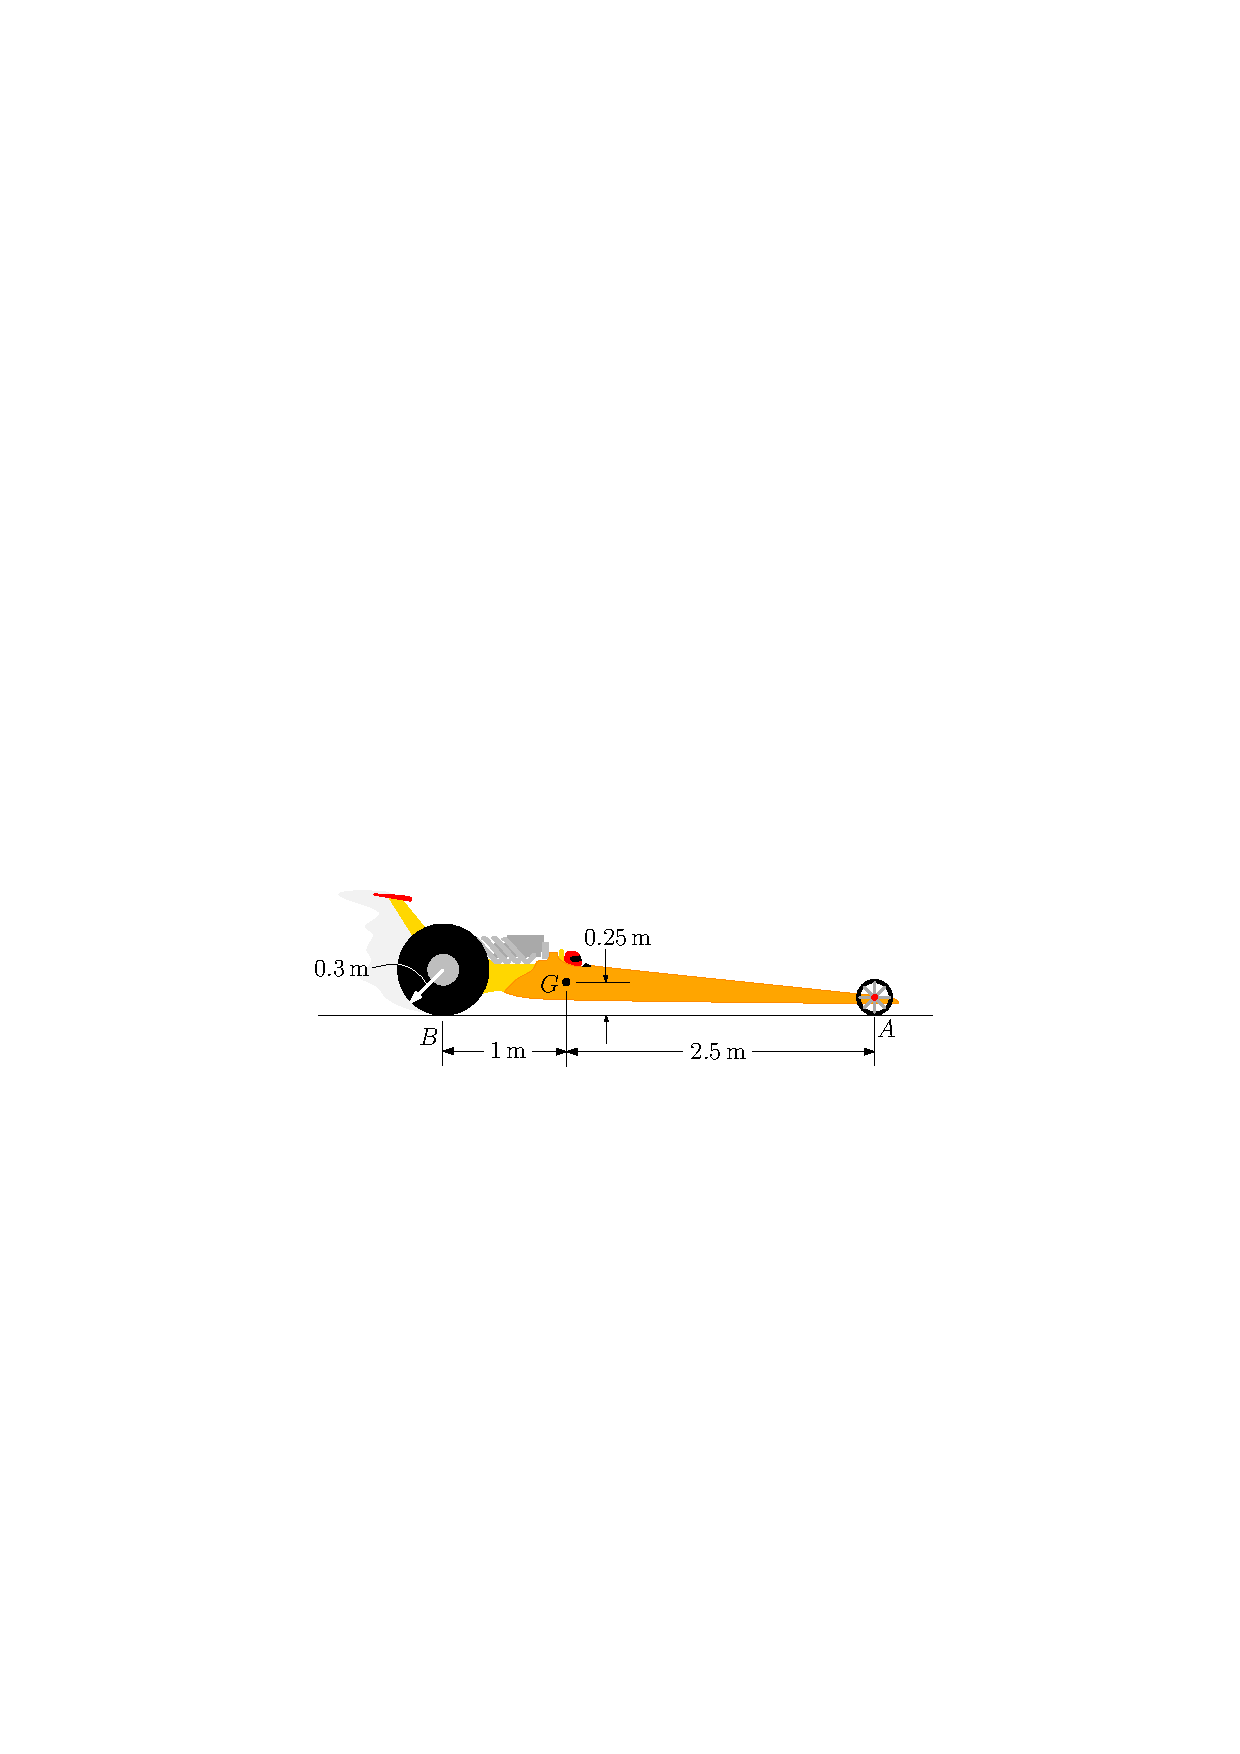
\includegraphics[scale=1]{../../images/draw_5}
\end{flushleft}